%% LaTeX-Beamer template for KIT design
%% by Erik Burger, Christian Hammer
%% title picture by Klaus Krogmann
%%
%% version 2.1
%%
%% mostly compatible to KIT corporate design v2.0
%% http://intranet.kit.edu/gestaltungsrichtlinien.php
%%
%% Problems, bugs and comments to
%% burger@kit.edu

\documentclass[18pt]{beamer}
\usepackage[utf8x]{inputenc}
\usepackage{units}
\usepackage{booktabs}

%% CUSTOM
\usepackage{amsmath}
\usepackage{algpseudocode}

%% Definitions
\DeclareMathOperator{\div2}{div}
\renewcommand{\algorithmicrequire}{\textbf{Input:}}
\renewcommand{\algorithmicensure}{\textbf{Output:}}
\algnewcommand\algorithmicto{\textbf{to}}
\algrenewtext{For}[3]{\algorithmicfor\ $#1 \gets #2$ \algorithmicto\ $#3$ \algorithmicdo}
\algnewcommand\algorithmicod{\textbf{od}}
\algrenewtext{EndWhile}{\algorithmicod}
\algrenewtext{EndFor}{\algorithmicod}
%\AtBeginSection[]{%
%\begin{frame}<beamer> % do nothing in handouts
%    \frametitle{Überblick}
%    \tableofcontents[sectionstyle=show/shaded,
%    subsectionstyle=show/show/hide]
%\end{frame}
%}
%\AtBeginSubsection[]{%
%\begin{frame}<beamer> % do nothing in handouts
%    \frametitle{Überblick}
%    \tableofcontents[sectionstyle=show/shaded,
%    subsectionstyle=show/shaded/hide]
%\end{frame}
%}

%% SLIDE FORMAT

% use 'beamerthemekit' for standard 4:3 ratio
% for widescreen slides (16:9), use 'beamerthemekitwide'

\usepackage{templates/beamerthemekit}
%\usepackage{templates/beamerthemekitwide}

 %% TITLE PICTURE

 % if a custom picture is to be used on the title page, copy it into the 'logos'
 % directory, in the line below, replace 'mypicture' with the 
 % filename (without extension) and uncomment the following line
 % (picture proportions: 63 : 20 for standard, 169 : 40 for wide
 % *.eps format if you use latex+dvips+ps2pdf, 
 % *.jpg/*.png/*.pdf if you use pdflatex)


 \titleimage{banner}
 
 
%% Define some colors:
\definecolor{darkblue}{rgb}{0,0,.5}
\definecolor{darkgreen}{rgb}{0,.5,0}

 %% TITLE LOGO

 % for a custom logo on the front page, copy your file into the 'logos'
 % directory, insert the filename in the line below and uncomment it

\titlelogo{logo_150x150}
 
 % (*.eps format if you use latex+dvips+ps2pdf,
 % *.jpg/*.png/*.pdf if you use pdflatex)
 
 %% TikZ INTEGRATION
 
 % use these packages for PCM symbols and UML classes
 % \usepackage{templates/tikzkit}
 % \usepackage{templates/tikzuml}
 
 % the presentation starts here
 
\author{Dominik Muth - dominik.muth@student.kit.edu}
\institute{Institut f\"ur Informatik}

\subtitle{Foliensatz 8}
\date{13. Dezember 2012}

\begin{document}

\begin{frame}
    \titlepage
\end{frame}

\begin{frame}{Outline/Gliederung}
    \tableofcontents
\end{frame}

\section{Übungsblatt 8}
\begin{frame}{Allgemeine Fehler, Fragen}
    \begin{block}{Allgemeines}
        \begin{itemize}
        \end{itemize}
    \end{block}
\end{frame}

\section{Wiederholung}
\begin{frame} {Wiederholung - Quiz}
    \begin{itemize}
        \item In jedem gerichteten Baum gibt es genau einen Knoten $x_0$ mit
$d^{+}(x_0) = 0 \land d^{−}(x_0) \geq 0$
        \only<2-> {\color{darkgreen}$\surd$}\\
        \color{black}
        
        \item Zwischen zwei isomorphen Graphen gibt es immer nur einen Isomorphismus
        \only<3-> {\color{red}$X$}\\
        \color{black}
    \end{itemize}
\end{frame}

\section{Adjazenz}
\begin{frame}{Definition}
    \begin{block}{Adjazenz}
        Zwei Knoten $x$ und $y$ eines Graphen sind \emph{adjazent} (oder \emph{benachbart}), wenn sie durch eine Kante verbunden sind.
    \end{block}
\end{frame}
\begin{frame}{Adjazenzliste}
    \begin{block}{Definition}
        In der Adjazenzliste stehen zu einem Knoten $x$ alle Knoten $y$, die von $x$ direkt erreichbar sind.
    \end{block}
\end{frame}
\begin{frame}{Adjazenzliste - Beispiel}
    \begin{columns}
        \begin{column}{.5\textwidth}
            \centering
            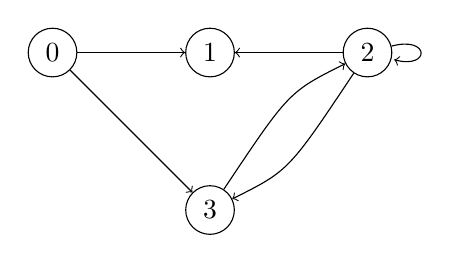
\begin{tikzpicture}
              \tikzstyle{every node}=[draw,shape=circle];
                \path[fill] (0,0)  node[circle] (0) {0};
                \path[fill] (2,0)  node[circle] (1) {1};
                \path[fill] (4,0)  node[circle] (2) {2};
                \path[fill] (2,-2) node[circle] (3) {3};

                \path[->,draw] (0) -- (1);
                \path[->,draw] (2) -- (1);
                \path[->,draw] (2) edge [loop right] ();
                \path[->,draw] (3).. controls (3,-0.5)..  (2);
                \path[->,draw] (2).. controls (3,-1.5)..  (3);
                \path[->,draw] (0) -- (3);
            \end{tikzpicture}
        \end{column}
        \begin{column}{.5\textwidth}
            \begin{table}
                \begin{tabular}{|l|l|}
                    \hline
                    0 & 1,2\\\hline
                    1 & \\\hline
                    2 & 1,2,3\\\hline
                    3 & 2\\\hline
                \end{tabular}
            \end{table}
        \end{column}
    \end{columns}
\end{frame}
\begin{frame}{Ajazenzmatrix}
    \begin{block}{Definition}
        Bei einem Graphen mit $n$ Knoten bezeichnet die Matrix $A \in\left\{ 0,1 \right\}^n \times \left\{ 0,1 \right\}^n$ die Adjazenmatrix des Graphen. Für die Matrix gilt:
        \begin{align*}
            A_{ij} = \begin{cases}
                0 & \left( i,j \right) \notin E\\
                1 & \left( i,j \right) \in E
            \end{cases}
        \end{align*}
    \end{block}
\end{frame}
\begin{frame}{Adjazenzmatrix - Beispiel}
    \begin{columns}
        \begin{column}{.5\textwidth}
            \centering
            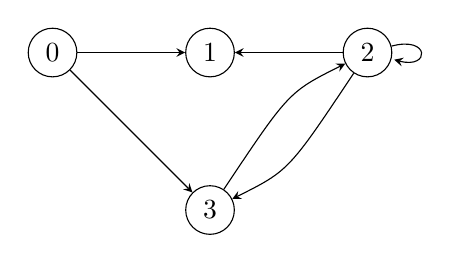
\begin{tikzpicture}[->,>=stealth,baseline=-5mm]
              \tikzstyle{every node}=[draw,shape=circle];
                \path[fill] (0,0)  node[circle] (0) {0};
                \path[fill] (2,0)  node[circle] (1) {1};
                \path[fill] (4,0)  node[circle] (2) {2};
                \path[fill] (2,-2) node[circle] (3) {3};

                \path[->,draw] (0) -- (1);
                \path[->,draw] (2) -- (1);
                \path[->,draw] (2) edge [loop right] ();
                \path[->,draw] (3).. controls (3,-0.5)..  (2);
                \path[->,draw] (2).. controls (3,-1.5)..  (3);
                \path[->,draw] (0) -- (3);
            \end{tikzpicture}
        \end{column}
        \begin{column}{.5\textwidth}
            A = \begin{pmatrix}
                0& 1& 0& 1\\
                0& 0& 0& 0\\
                0& 1& 1& 1\\
                0& 0& 1& 0
            \end{pmatrix}
        \end{column}
    \end{columns}
\end{frame}
\begin{frame}{Adjazenzmatrix - Beispiel 2}
    \begin{columns}
        \begin{column}{.5\textwidth}
            \centering
            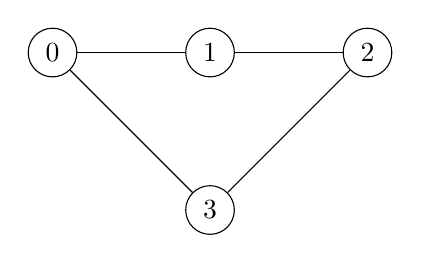
\begin{tikzpicture}[-,>=stealth,baseline=-5mm]
              \tikzstyle{every node}=[draw,shape=circle];
                \path[fill] (0,0)  node[circle] (0) {0};
                \path[fill] (2,0)  node[circle] (1) {1};
                \path[fill] (4,0)  node[circle] (2) {2};
                \path[fill] (2,-2) node[circle] (3) {3};

                \path[-,draw] (0) -- (1);
                \path[-,draw] (2) -- (1);
                \path[-,draw] (3) -- (2);
                \path[-,draw] (0) -- (3);
            \end{tikzpicture}
        \end{column}
        \begin{column}{.5\textwidth}
            A = \begin{pmatrix}
                0& 1& 0& 1\\
                1& 0& 1& 0\\
                0& 1& 0& 1\\
                1& 0& 1& 0
            \end{pmatrix}
        \end{column}
    \end{columns}
\end{frame}
\begin{frame}{Besondere Adjazenzmatrizen}
    \begin{columns}
        \begin{column}{.5\textwidth}
            \begin{align*}
                A = \begin{pmatrix}
                    1 & 1 & 1\\
                    1 & 1 & 1\\
                    1 & 1 & 1
                \end{pmatrix}
            \end{align*}
        \end{column}
        \begin{column}{.5\textwidth}
            Einheitsmatrix:
            \begin{align*}
                \mathbb{I} = \begin{pmatrix}
                    1 & 0 & 0\\
                    0 & 1 & 0\\
                    0 & 0 & 1
                \end{pmatrix}
            \end{align*}
        \end{column}
    \end{columns}
\end{frame}
\begin{frame}{Adjazenzmatrix - Eigenschaften}
    \begin{itemize}
        \item Schlingen stehen bei $A_{ii}$
        \item Ungerichteter Graph $\Leftrightarrow$ $A$ symmetrisch $\Leftrightarrow$ $A_{ij} = A_{ji}$
    \end{itemize}
\end{frame}
\begin{frame}{Vergleich: Adjazenzmatrix und Adjazenzliste}
    \begin{columns}
        \begin{column}{.5\textwidth}
            \begin{itemize}
                \item Spart Speicherplatz (bei wenig Kanten)
                \item Schneller Zugriff auf adjazente (``benachbarte'') Knoten
            \end{itemize}
        \end{column}
        \begin{column}{.5\textwidth}
            \begin{itemize}
                \item Konstanter Speicherplatzverbrauch $n^2$
                \item Schneller Zugriff auf Kante von $i$ nach $j$
                \item Komfortabel auch bei vielen Kanten
            \end{itemize}
        \end{column}
    \end{columns}
\end{frame}
\begin{frame}{Potenz der Adjazenzmatrix}
    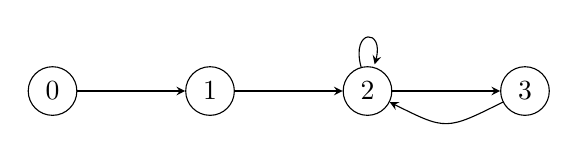
\begin{tikzpicture}[->,>=stealth]
      \tikzstyle{every node}=[draw,shape=circle];
        \path[fill] (0,0)  node[circle] (0) {0};
        \path[fill] (2,0)  node[circle] (1) {1};
        \path[fill] (4,0)  node[circle] (2) {2};
        \path[fill] (6,0)  node[circle] (3) {3};

        \path[->,draw] (0) -- (1);
        \path[->,draw] (1) -- (2);
        \path[->,draw] (2) edge [loop above] ();
        \path[->,draw] (3).. controls (5,-0.5)..  (2);
        \path[->,draw] (2) -- (3);
    \end{tikzpicture}
    \begin{columns}
        \begin{column}{.5\textwidth}
            \begin{align*}
                A = \begin{pmatrix}
                    0 & 1 & 0 & 0\\
                    0 & 0 & 1 & 0\\
                    0 & 0 & 1 & 1\\
                    0 & 0 & 0 & 0
                \end{pmatrix}
            \end{align*}
        \end{column}
        \begin{column}{.5\textwidth}
            \begin{align*}
                A^2 = \begin{pmatrix}
                    \visible<2->{0 & 0 & 1 & 0\\
                    0 & 0 & 1 & 1\\
                    0 & 0 & 1 & 1\\
                    0 & 0 & 0 & 0}
                    \end{pmatrix}
            \end{align*}
        \end{column}
    \end{columns}
    \visible<3->{$\left( A^2 \right)_{ij}$ gibt Auskunft, ob es einen \emph{Weg der Länge 2} von $i$ nach $j$ gibt}
\end{frame}
\begin{frame}{Matrixmultiplikation}
    Berechne jeweils $AB$ und $BA$.
    \begin{columns}
        \begin{column}{.5\textwidth}
            \begin{align*}
                A = \begin{pmatrix}
                    1 & 1 & 1 & 1\\
                    0 & 1 & 1 & 1\\
                    0 & 0 & 1 & 1\\
                    0 & 0 & 0 & 1
                \end{pmatrix}
            \end{align*}
        \end{column}
        \begin{column}{.5\textwidth}
            \begin{align*}
                B = \begin{pmatrix}
                    0 & 0 & 0 & 0\\
                    1 & 0 & 0 & 0\\
                    1 & 1 & 0 & 0\\
                    1 & 1 & 1 & 0
                    \end{pmatrix}
            \end{align*}
        \end{column}
    \end{columns}
    \visible<2->{Lösung:
    \begin{columns}
        \begin{column}{.5\textwidth}
            \begin{align*}
                AB = \begin{pmatrix}
                    3 & 2 & 1 & 0\\
                    3 & 2 & 1 & 0\\
                    2 & 2 & 1 & 0\\
                    1 & 1 & 1 & 0
                \end{pmatrix}
            \end{align*}
        \end{column}
        \begin{column}{.5\textwidth}
            \begin{align*}
                BA = \begin{pmatrix}
                    0 & 0 & 0 & 0\\
                    1 & 1 & 1 & 1\\
                    1 & 2 & 2 & 2\\
                    1 & 2 & 3 & 3
                    \end{pmatrix}
            \end{align*}
        \end{column}
    \end{columns}}
\end{frame}
\begin{frame}{Matrixmultiplikation - Algorithmus}
    \begin{algorithm}
        \begin{algorithmic}
            \For{i}{0}{l-1}
                \For{j}{0}{m-1}
                    \State $C_{ij}\gets 0$
                    \For{k}{0}{n-1}
                    \State $C_{ij}\gets C_{ij} + A_{ik}\cdot B_{kj}$
                    \EndFor
                \EndFor
            \EndFor
        \end{algorithmic}
    \end{algorithm}
\end{frame}
\begin{frame}{Die Einheitsmatrix}
    \begin{columns}
        \begin{column}{.5\textwidth}
            $3\times 3$-Einheitsmatrix:
            \begin{align*}
                \mathbb{I} = \begin{pmatrix}
                    1 & 0 & 0\\
                    0 & 1 & 0\\
                    0 & 0 & 1
                \end{pmatrix}
            \end{align*}
        \end{column}
        \begin{column}{.5\textwidth}
            \begin{align*}
                A\mathbb{I} = \mathbb{I}A = A
            \end{align*}
        \end{column}
    \end{columns}
\end{frame}
\begin{frame}{Wegematrix}
    \begin{block}{Definition}
        Die Wegematrix $W$ ist definiert als
        \begin{align*}
            W_{ij} = \begin{cases} 0 & \left( i,j \right) \notin E^*\\
                1 & \left( i,j \right) \in E^*\end{cases}
        \end{align*}
        Ein Algorithmus zur Berechnung ist
        \begin{align*}
            W_{ij} = \sgn\left( \left( \sum_{k=0}^{n}A^k \right)_{ij} \right)
        \end{align*}
        Dabei ist $\sgn$ die ``Vorzeichenfunktion'':
        \begin{align*}
            \sgn\left( x \right) = \begin{cases} + 1& x>0\\
                0 & x=0\\
                -1 & x<0\end{cases}
        \end{align*}
    \end{block}
\end{frame}
\begin{frame}{Eigenschaften der Wegematrix}
    \begin{itemize}
        \item Die Wegematrix ist die Adjazenzmatrix der reflexiv-transitive Hülle
        \item Gibt es einen beliebigen Weg zwischen zwei Knoten $i$ und $j$, ist $W_{ij} = 1$.
    \end{itemize}
\end{frame}
\begin{frame}{Der einfache Algorithmus zur Wegematrix}
    \begin{algorithm}
        \begin{algorithmic}
            \State $W \gets 0$ \Comment{Nullmatrix}
            \For{i}{0}{n-1}
                \State $M \gets \mathbb{I}$ \Comment{Einheitsmatrix}
                \For{j}{1}{i}
                    \State $M \gets M\cdot A$
                \EndFor
                \State $W \gets W + M$ 
            \EndFor
            \State $W \gets \sgn\left( W \right)$
        \end{algorithmic}
    \end{algorithm}
\end{frame}
\begin{frame}{Eigenschaften des Algorithmus}
    \begin{itemize}
        \item $A^n$ macht $\sum_{i=0}^{n-1} i =  \frac{n\left( n-1 \right)}{2}$ Matrixmultiplikationen
        \item Jede Matrixmultiplikation macht $n^2$ Operationen
        \item Summe: $n^2$ Matrixelemente addieren, das ganze $n$ Mal: Über $n\Rightarrow n\cdot n^2 = n^3$ Operationen
        \item Signum-Funktion: $n^2$ Operationen
    \end{itemize}
    \begin{align*}
        \Rightarrow n^2 + n^3 + n^2\left( n + n - 1 \right)\cdot\frac{n\left( n-1 \right)}{2} = n^5 + \mathcal{0}\left( n^4 \right)
    \end{align*}
    Algorithmuslaufzeit: $n^5$
\end{frame}
\begin{frame}{Laufzeitverbesserung}
    Wie könnte Laufzeit gespart werden (eventuell mit mehr Speicherverbrauch)? \visible<2->{Etwa durch Zwischenspeichern der berechneten Matrizen $A^i$.}\\
    Vergleich der Algorithmen:
    \begin{columns}
        \begin{column}{.5\textwidth}
            \begin{algorithm}
                \begin{algorithmic}
                    \State $W \gets 0$ \Comment{Nullmatrix}
                    \For{i}{0}{n-1}
                        \State $M \gets \mathbb{I}$ \Comment{Einheitsmatrix}
                        \For{j}{1}{i}
                            \State $M \gets M\cdot A$
                        \EndFor
                        \State $W \gets W + M$ 
                    \EndFor
                    \State $W \gets \sgn\left( W \right)$
                \end{algorithmic}
            \end{algorithm}
        \end{column}
        \visible<3->{\begin{column}{.5\textwidth}
            \begin{algorithm}
                \begin{algorithmic}
                    \State $W \gets 0$ \Comment{Nullmatrix}
                    \State $M \gets \mathbb{I}$ \Comment{Einheitsmatrix}
                    \For{i}{0}{n-1}
                        \State $W \gets W + M$ 
                        \State $M \gets M\cdot A$
                    \EndFor
                    \State $W \gets \sgn\left( W \right)$
                \end{algorithmic}
            \end{algorithm}
        \end{column}}
    \end{columns}
\end{frame}

\begin{frame}{Der $n^4$-Algorithmus}
    \begin{algorithm}
        \begin{algorithmic}
            \State $W\gets A + \mathbb{I}$
            \State $m \gets \log_2\left( n \right)$
            \For{i}{1}{m}
                \State $W \gets W\cdot W$
            \EndFor
            \State $W\gets \sgn\left( W \right)$
        \end{algorithmic}
    \end{algorithm}
    Wie sieht das mit der Laufzeit aus?
\end{frame}

\begin{frame}{Der Algorithmus von Warshall}
    \begin{columns}
        \begin{column}{.5\textwidth}
            \begin{algorithm}
                \begin{algorithmic}
                    \For{i}{0}{n-1}
                        \For{j}{0}{n-1}
                        \State $W_{ij} \gets \begin{cases} 1 & \text{falls } i = j\\
                            A_{ij} & \text{falls } i\neq j\end{cases}$
                        \EndFor
                    \EndFor
                    \For{k}{0}{n-1}
                        \For{i}{0}{n-1}
                            \For{j}{0}{n-1}
                                \State $W_{ij} \gets \max\left( W_{ij}, \min\left( W_{ik},W_{kj} \right) \right)$
                            \EndFor
                        \EndFor
                    \EndFor
                    \State $W \gets \sgn\left( W \right)$
                \end{algorithmic}
            \end{algorithm}
        \end{column}
        \begin{column}{.5\textwidth}
            Beispiel: Berechne die Wegematrix für
                \begin{align*}
                    G = \left( &\left\{ 0,1,2,3 \right\},\\&\left\{ \left( 0,3 \right),\left( 1,0 \right),\left( 2,3 \right),\left( 3,1 \right) \right\} \right)
                \end{align*}
       \end{column}
    \end{columns}
\end{frame}

\section{Aufgabe}
\begin{frame}{Beispiel}
    Gegeben sei die Adjazenzliste:
    \begin{table}
        \centering
        \begin{tabular}{|l|l|}
            \hline
            0 & 1,  2\\\hline
            1 & \\\hline
            2& 0, 3, 5\\\hline
            3 & 0\\\hline
            4 & 2, 4\\\hline
            5 & 1, 3, 4\\\hline
        \end{tabular}
    \end{table}
    Bilde die Adjazenzmatrix und die Wegematrix mit dem Warshall-Algorithmus.
\end{frame}
\begin{frame}{Aufgabe 2}
    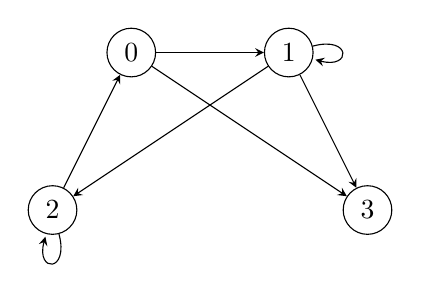
\begin{tikzpicture}[->,>=stealth]
      \tikzstyle{every node}=[draw,shape=circle];
        \path[fill] (1,2)  node[circle] (0) {0};
        \path[fill] (3,2)  node[circle] (1) {1};
        \path[fill] (0,0)  node[circle] (2) {2};
        \path[fill] (4,0)  node[circle] (3) {3};

        \path[->,draw] (0) -- (1);
        \path[->,draw] (0) -- (3);
        \path[->,draw] (1) edge [loop right] ();
        \path[->,draw] (1) -- (2);
        \path[->,draw] (1) -- (3);
        \path[->,draw] (2) edge [loop below] ();
        \path[->,draw] (2) -- (0);
    \end{tikzpicture}


    Geben Sie
    \begin{itemize}
        \item die Adjazenliste,
        \item die Adjazenzmatrix,
        \item die Wegematrix,
        \item und die Zwischenmatrizen beim Berechnen der Wegematrix mit dem Warshall-Algorithmus
    \end{itemize}
    an.
\end{frame}

\end{document}
